\documentclass[10pt,a4paper]{article}
\usepackage{geometry}
\usepackage[french]{babel}
\usepackage[utf8]{inputenc}
\usepackage[T1]{fontenc}
\usepackage{lmodern} \normalfont
\DeclareFontShape{T1}{lmr}{bx}{sc}{<-> ssub * cmr/bx/sc}{}
\usepackage{textcomp}
\usepackage{datetime}
\usepackage{amsmath}
\usepackage{amssymb}
\usepackage{graphicx}
\usepackage{wrapfig}
\usepackage{subcaption}
\usepackage{tocloft}
\usepackage{fixltx2e}
\usepackage{color}
\usepackage[colorlinks=true,
			linkcolor=blue,
			bookmarksnumbered=true,
			pdftitle={Rapport de stage},
			pdfauthor={Gwenegan Hudin},
			pdfborder={0 0 0},
			pdfsubject={Stage 3INFO}]{hyperref}

% Custom commands
\newcommand{\HRule}{\rule{\linewidth}{0.5mm}}
\newcommand{\Section}[1]{\section*{#1} \addcontentsline{toc}{section}{#1} \setcounter{subsection}{0}}
%\renewcommand*{\theHsection}{chY.\the\value{section}}
\renewcommand{\thesection}{\Roman{section}.}
\renewcommand{\thesubsection}{\arabic{subsection}.}
\renewcommand{\thesubsubsection}{\alph{subsubsection}.}
\renewcommand{\cftsecnumwidth}{2em}
\renewcommand{\cftsubsecnumwidth}{2em}
\renewcommand{\cftsubsubsecnumwidth}{2em}
\addto\captionsfrench{
	\renewcommand{\cfttoctitlefont}{\Large}
	\renewcommand{\contentsname}{\centering \textsc{Table des Matières}\\[0.5cm]}
}

\renewcommand{\baselinestretch}{1.15}

\begin{document}

\begin{titlepage}
	\begin{center}
		\begin{figure}
        \begin{subfigure}[c]{0.2\textwidth}
        		\centering
                
\includegraphics[width=0.6\textwidth]{images/logo-polymtl}
        \end{subfigure}
		\end{figure}
		
		
		\vspace{30pt}
		\textsc{\huge Génie Informatique}\\
		\textsc{\LARGE Rapport de Travaux Pratiques}\\		
		\vfill
		
		% Title
		\HRule \\[0.7cm]
		{\Huge \bfseries INF4705 : Lab 1}\\[0.4cm]
		{\Large Algorithmes Diviser-pour-régner : Application à la multiplication de matrices carrées}\\[0.2cm]
		\HRule\\[1cm]
		
		\vfill
		
		% Author
		\begin{minipage}{0.49\textwidth}
			\begin{flushleft} \LARGE
				\textbf{Auteur}\\
				Gwenegan \textsc{Hudin}\\ 1756642\\[0.5cm]
			\end{flushleft}
		\end{minipage}
		\begin{minipage}{0.49\textwidth}
			\begin{flushright} \LARGE
				\textbf{Rendu}\\
				10 Octobre 2014\\ À Polytechnique Montréal\\[0.5cm]
			\end{flushright}
		\end{minipage}
	\end{center}
\end{titlepage}

\newpage

\hfill

\newpage

\tableofcontents

\newpage

\section{Introduction}

Les algorithmes dits \og diviser-pour-régner \fg désignent un patron de conception algorithmique dans lequel le problème visé est subdivisé en une séries de problèmes moins complexes dont les solutions sont utilisées pour déterminer celle du problème original. Nous allons dans cette expérience étudier l'intérêt de l'algorithme de multiplication de matrices carrées de Strassen contre la méthode de calcul conventionnel, dite \og naïve \fg.

Ce faisant, nous voulons démontrer qu'une utilisation réfléchie d'un algorithme diviser-pour-régner, dans de bonnes conditions d'application (qui seront déterminées par l'expérience), est plus efficace en termes de temps que l'algorithme conventionnel. Rappelons brièvement que l'algorithme de Strassen subdivise en quatre ses deux opérandes tant que leur taille est supérieure à un certain seuil, en deçà duquel la multiplication conventionnelle est calculée. Les conditions sus-citées sont donc la taille des matrices à multiplier, et le seuil appliqué.

L'on suppose que la méthode conventionnelle sera la plus efficace uniquement sur des matrices de taille faible, ainsi que sur toute matrice lorsque la méthode de Strassen est appliquée avec un seuil trop faible ou trop important. L'on suppose aussi que la méthode de Strassen, appliquée avec un seuil supérieur à la taille de la matrice, obtiendra des résultats comparables à ceux de la méthode naïve.

Ce rapport a pour but de mettre en pratique les méthodes d'analyse empirique et hybride d'algorithmes, et de présenter les résultats de l'expérience conduite.

\section{Revue de la théorie}
\subsection{Fonctionnement de l'algorithme de Strassen}

La méthode diviser-pour-régner de Strasse consiste à :

\begin{itemize}
	\item Découper chacune des deux matrices en quatre parties égales
	\item Effectuer sept opérations scalaires avec ces huit matrices
	\item Recombiner les sept résultats en quatre matrices
	\item Fusionner ces quatre matrices en une matrice résultat
\end{itemize}

On remarque que lors de la deuxième étape, il est nécessaire d'effectuer de nouveau des multiplications de matrices. C'est ici que le seuil évoqué précédemment intervient : tant que les matrices ont une taille supérieure ou égale au double du seuil (donc toujours supérieure ou égale au seuil après découpage), on appelle récursivement cette méthode sur les sept opérations scalaires. Sinon, on les effectue selon la méthode conventionnelle.

L'étape de recombinaison se fait seulement par additions et soustractions. La découpe et la fusion dépendent fortement de l'implémentation et présentent plus de problématiques de complexité spatiale que temporelle.

\subsection{Étude de sa complexité}

Soit $ n $ la taille des matrices considérées. Soit $ T(n) $ la complexité temporelle de la multiplication.

Écartons de suite les étapes de découpage et fusion. Dans l'implémentation considérée, le découpage consiste en un simple parcours de chaque matrice, et affectation de chaque élément dans une nouvelle matrice, soit $ \theta (2n^{2}) $ pour chacune des deux matrices, donc $ \theta (4n^{2}) $ pour les deux. L'étape 1 appartient donc à $ \theta (n^{2}) $. De même, la fusion consiste en un parcours de quatre matrices de taille $ \frac{n}{2} $ et affectation, appartenant ainsi à $ \theta (n^{2}) $.

Comme l'accès et l'affectation, la soustraction et l'addition sont considérées comme étant des opérations élémentaires. Selon la formule de combinaison de Strassen, chacune des quatre sous-matrices est le résultat d'additions et soustractions de deux ou quatre matrices de taille $ \frac{n}{2} $. Cette étape s'exprime donc aussi dans $ \theta (n^{2}) $.

Enfin, la deuxième étape est composée de sept nouvelles multiplications, sur des matrices de taille $ \frac{n}{2} $, et s'effectuent donc en temps $ 7T( \frac{n}{2}) $. Nous pouvons donc en déduire que la complexité temporelle de l'algorithme de Strassen s'exprime ainsi : $ T(n) \leq 7T( \frac{n}{2}) + Cn^{2} $.

On notera que la complexité de l'algorithme conventionnel s'exprime dans $ \theta (n^{3}) $.

\section{Protocole expérimental}

\subsection{Environnement de développement}

Les tests ont été effectués sur un système ArchLinux 64bits, kernel 3.16.3-1-ARCH en environnement Gnome3, sur une machine disposant de 8Go de mémoire vive et d'un processeur i7-2630QM cadencé à 2.00GHz. L'ordinateur portable a reposé sur une station ventilée pendant toute la durée des calculs.

Le programme a été écrit en C++ 11 et compilé avec GCC 4.9.1.

\subsection{Déroulement de l'expérience}

Un soin tout particulier a été apporté à la rédaction du code qui est voulu lisible et efficace. Une fois les deux algorithmes implémentés, la validité des calculs de la méthode de Strassen a été vérifiée sur des exemplaires de taille $ 2^{5} $ et $ 2^{10} $, avec des seuils en $ 2^{x} $ ($ x $ de 0 à 7).

L'égalité entre le résultat de la multiplication naïve, que l'on prend comme résultat de référence du fait de la simplicité de son implémentation, et le résultat de la méthode de Strassen a été vérifiée pour ces jeux de données et ces différents seuils. Ceci a permis d'écarter plusieurs erreurs d'implémentation de l'algorithme de Strassen et assurer des résultats cohérents et valides avant de considérer tous les jeux de tests, dont le calcul est coûteux.

Ensuite, le seuil optimal a été déterminé par tâtonnement, en essayant  des seuils de $ 2^{1} $ à $ 2^{7} $ et en comparant avec les résultats obtenus par le calcul conventionnel. Ces essais ont porté sur toutes les tailles de matrices proposées, soit de $ 2^{5} $ à $ 2^{10} $.

Une fois le seuil optimal obtenu, cinq exécutables ont été créés, permettant d'effectuer un calcul conventionnel ou un calcul de Strassen avec un seuil optimal, tiers d'optimal, triple d'optimal et égal à 1. Tous ces exécutables ont été utilisés pour effectuer tous les calculs de chaque exemplaire, par scripting Bash, et stocker leurs résultats dans des fichiers texte. Ainsi, pour chacun des exécutables, pour chaque taille de matrice, 10 calculs ont été effectués et leur temps consigné.

Ces temps ont ensuite été reportés dans LibreOffice Calc pour analyse.

\section{Résultats}

Suite aux tests par tâtonnement, et après discussion avec différents groupes, le seuil optimal de l'algorithme de Strassen a été fixé à 64, soit $ 2^{6} $. Par la suite, on fera référence à l'exécutable opérant selon cette méthode avec seuil 64 comme "Strassen 64", et de façon similaire pour les autres exécutables (Tiers, Triple, Un).

Après avoir reporté et moyenné les dix résultats pour les cinq tailles d'exemplaires calculés avec cinq exécutables différents, les données sont probantes.

\begin{figure}[h!]
	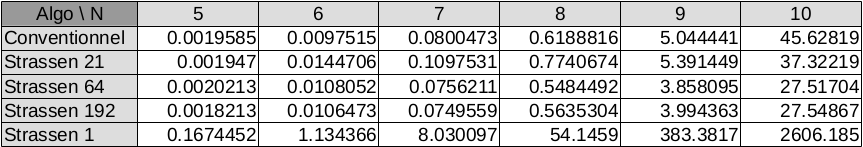
\includegraphics[width=\textwidth]{spreadsheet/times}
	\caption{Table des moyennes des temps de calculs, exprimées en secondes}
\end{figure}

Ces mesures sont cohérentes et ne présentent pas d'anomalie. Cependant, dans les figures qui suivent, les résultats de Strassen 1 ne sont pas inclus, et ce afin de ne pas perturber la lecture par un changement d'échelle trop important dû à ses mauvais résultats.

\begin{figure}[h!]
	\centering
	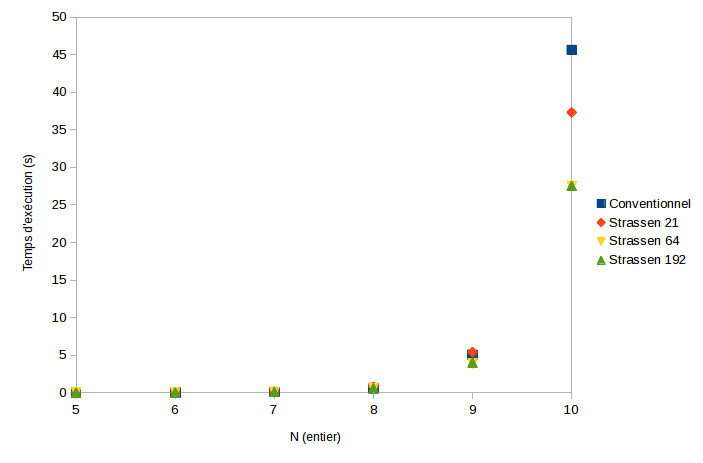
\includegraphics[width=0.9\textwidth]{spreadsheet/graph1}
	\caption{Représentation graphique des moyennes de temps de calcul}
\end{figure}

Sur lq Figure 3, l'on peut aisément constater que l'algorithme naïf est dépassé à partir de $ N = 9 $, suivi par Strassen Tiers. On ne peut cependant pas encore tirer de conclusions sur les seuils inférieurs sans faire de zoom.

\begin{figure}[h!]
	\begin{subfigure}[c]{0.5\textwidth}
		\centering
		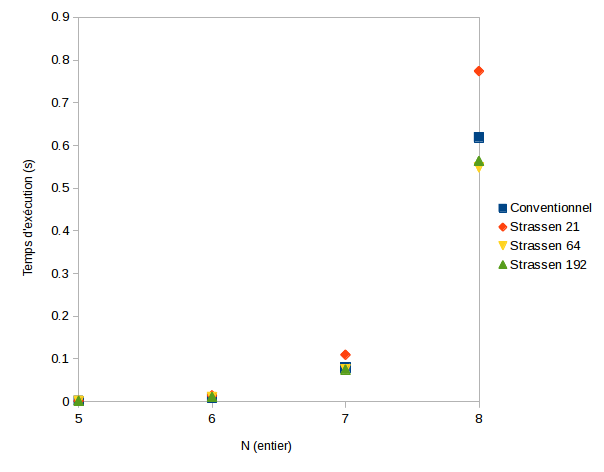
\includegraphics[width=\textwidth]{spreadsheet/graph2}
		\caption{Zoom sur N inférieur à 9 sur la Figure 3}
	\end{subfigure}
	\begin{subfigure}[c]{0.5\textwidth}
		\centering
		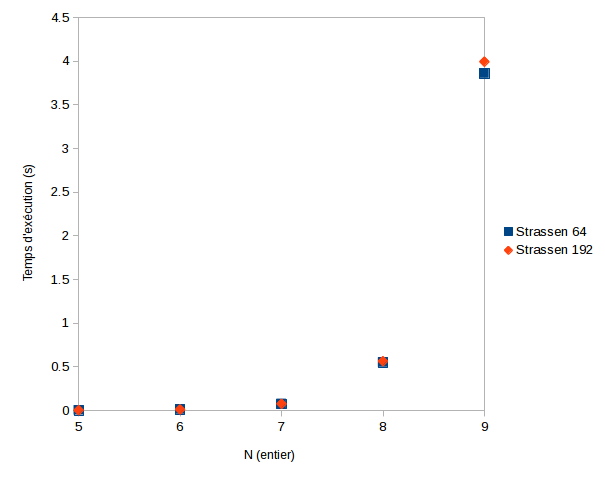
\includegraphics[width=\textwidth]{spreadsheet/graph3}
		\caption{Comparaison graphique Strassen Seuil et Triple pour N inférieur à 10}
	\end{subfigure}
	\caption{Zooms sur les données de temps de calcul}
\end{figure}

À travers ces représentations à plus petite échelle, on constate que pour N à 5 et 6 les résultats sont indissociables. Pour N plus grand, Strassen Tiers est moins efficace que l'algorithme naïf (contrairement à ce que laissait penser le graphique en Figure 3), qui est lui même dépassé par Strassen Seuil et Triple, qui semblent se comporter de la même manière.

Leur comparaison plus poussée, sur N de 5 à 9, le corrobore. Pour N inférieur ou égal à 8, Strassen Seuil et Triple sont parfaitement similaires (sachant que ce n'est que pour $ N = 8 $ que Strassen Triple se différencie de Conventionnel), mais on peut constater une légère hausse d'efficacité pour Strassen Seuil à partir de $ N = 9 $.

Enfin, Strassen Un a été consigné dans un graphique à part, du fait de son inefficacité par rapport aux autres méthodes, pouvant atteindre 45 minutes de calcul pour $ N = 10 $. C'est donc cet exécutable qui a le plus ralenti la procédure de test, comme on peut voir sur la Figure 5.

\newpage

\begin{figure}[h!]
	\centering
	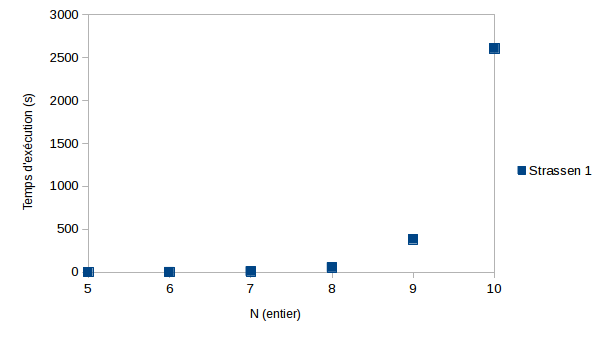
\includegraphics[width=0.9\textwidth]{spreadsheet/graph4}
	\caption{Représentation graphique des moyennes de temps de calcul pour Strassen Un}
\end{figure}

\newpage

\section{Analyse}

Pour l'analyse empirique des deux méthodes, on considère les couples $ (x,y) $, où $ x $ est la taille des matrices à multiplier, et $ y $ est le temps de calcul requis.

\subsection{Algorithme conventionnel}
\subsubsection{Test de puissance}

Lors de notre étude de la complexité de l'algorithme, nous avons évoqué sa complexité théorique en $ \theta (n^{3}) $, ce que nous allons vérifier. Nous effectuons d'abord le test de puissance en représentant $ y $ en fonction de $ x $ sur échelle log-log, sur la Figure 6.

\begin{figure}[h!]
	\centering
	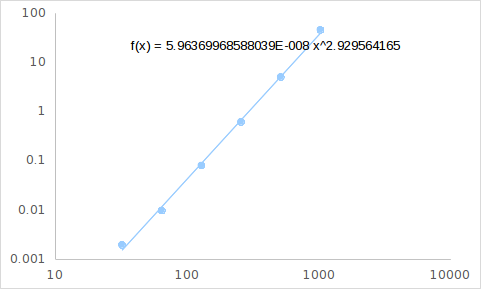
\includegraphics[width=0.75\textwidth]{spreadsheet/graph5}
	\caption{Test de puissance sur l'algorithme naïf, avec régression linéaire}
\end{figure}

La droite associée aux mesures indique une croissance polynomiale, avec un exposant proche de 2.92. Cela valide l'analyse théorique de l'algorithme, et l'on peut donc s'intéresser à la croissance cubique du temps de calcul pour l'algorithme naïf, que nous allons vérifier. 

\subsubsection{Test de rapport}

Pour vérifier que la complexité est cubique, on utilise un test de rapport avec comme fonction $ f(x) = x^{3} $. On regarde alors si la courbe du couple $ (x,  \frac{y}{x^{3}}) $ converge vers une constante supérieure à 0, comme illustré sur la Figure 7.

\newpage

\begin{figure}[h!]
	\centering
	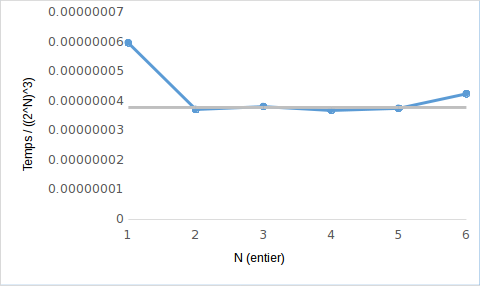
\includegraphics[width=0.75\textwidth]{spreadsheet/graph7}
	\caption{Test de rapport sur l'algorithme naïf, avec constante à $ 3.80 \cdot 10^{-8} $}
\end{figure}

Le graphique confirme que notre hypothèse est sensée, la courbe converge vers une constante proche de $ 3.80 \cdot 10^{-8} $.

\subsubsection{Test des constantes}

Pour ce dernier test, on représente $ f(x) $ en fonction de $ y $, soit la taille de la matrice au cube par le temps d'exécution du calcul. Les résultats sont reportés sur la Figure 8.

\begin{figure}[h!]
	\centering
	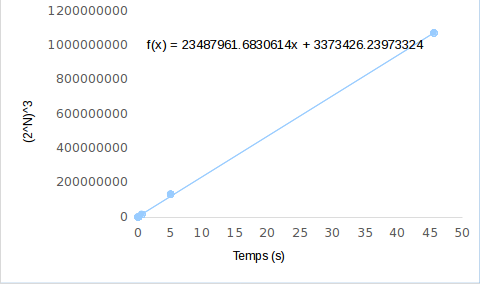
\includegraphics[width=0.75\textwidth]{spreadsheet/graph9}
	\caption{Test des constantes sur l'algorithme naïf, avec régression linéaire}
\end{figure}

Ici encore, la régression linéaire correspond aux données, avec une constante multiplicative de l'ordre de  $ 2.34 \cdot 10^{7} $ et un coût fixe de $ 3.37 \cdot 10^{6} $.

\subsection{Algorithme de Strassen}

Tous les tests évoqués précédemments ont aussi été appliqués à l'algorithme de Strassen, avec le seuil expérimental de 64. On rappelle que lors de l'analyse théorique, sa complexité s'exprimait en $ T(n) \leq 7T( \frac{n}{2}) + Cn^{2} $.

\subsubsection{Test de puissance}

Sur la Figure 9 ci-après est représenté le temps de calcul en fonction de la taille d'exemplaire à calculer, en échelle log-log.

\begin{figure}[h!]
	\centering
	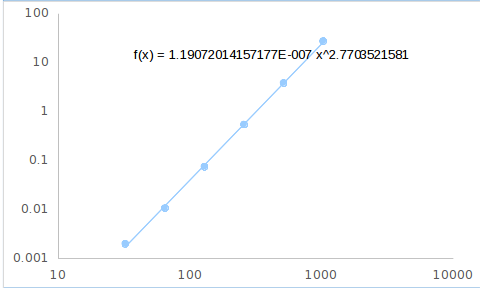
\includegraphics[width=0.75\textwidth]{spreadsheet/graph6}
	\caption{Test de puissance sur l'algorithme de Strassen, avec régression linéaire}
\end{figure}

Ici aussi, la droite correspond aux données, avec un exposant proche de 2.77. Afin d'être cohérents avec l'analyse vue en cours, nous allons considérer $ f(x) = x^{2.8} $ dans les prochains tests.

\subsubsection{Test de rapport}

Comme précédemment, on représente pour ce test le couple $ (x,  \frac{y}{x^{2.8}}) $, reporté ici sur la Figure 10.

\newpage

\begin{figure}[h!]
	\centering
	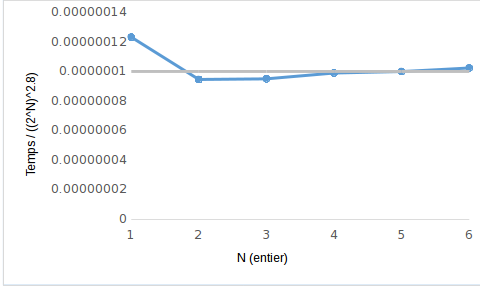
\includegraphics[width=0.75\textwidth]{spreadsheet/graph8}
	\caption{Test de rapport sur l'algorithme de Strassen, avec constante à $ 1.00 \cdot 10^{-7} $}
\end{figure}

La courbe converge vers la constante $ 1.00 \cdot 10^{-7} $, notre hypothèse est donc valide.

\subsubsection{Test des constantes}

Sur la Figure 11 est reportée la courbe représentant $ (2^{N})^{3} $ en fonction du temps de calcul.

\begin{figure}[h!]
	\centering
	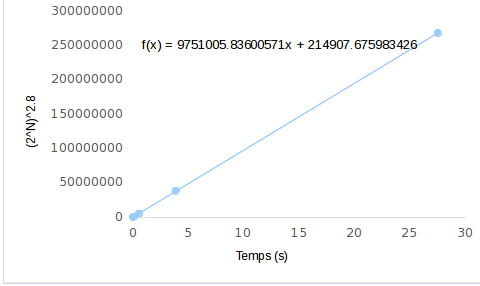
\includegraphics[width=0.75\textwidth]{spreadsheet/graph10}
	\caption{Test des constantes sur l'algorithme de Strassen, avec régression linéaire}
\end{figure}

La régression est correcte, avec une constante multiplicative de $ 9.75 \cdot 10^{6} $ et coût fixe de $ 2.15 \cdot 10^{5} $.

\subsection{Discussion}

\subsubsection{Choix du seuil}

L'expérience a montré que le choix du seuil utilisé par l'algorithme de Strassen était capital pour gagner en efficacité par rapport à la méthode de calcul naïve. Le seuil de 1 a des conséquences catastrophiques sur le temps de calcul, allant même jusqu'à compliquer la procédure de tests et de recueil de données, une seule multiplication pouvant prendre jusqu'à 45 minutes.

Le choix d'un seuil trop élevé, en revanche, porte bien moins à conséquences, car l'algorithme se comportera au pire comme la méthode naïve, en $ n^{3} $.

Le seuil impacte aussi quelles matrices seront concernées par la méthode diviser-pour-régner. Avec un seuil suffisamment haut, les matrices de taille plus faible seront immédiatement multipliées par la méthode naïve qui reste la plus efficace dans ce cas, sans aucune des opérations coûteuses supplémentaires amenées par la méthode de Strassen.

La sélection du seuil doit donc être réalisée avec grand soin et amplement testée, au risque de dégrader fortement les performances du programme.

\subsubsection{Conditions de choix d'algorithme}

Suite à ces analyses, il apparaît que le choix d'un des deux algorithmes tourne principalement autour de la taille des matrices à multiplier. Tant que des matrices de taille inférieure à 256 éléments étaient multipliées, la méthode de Strassen n'apportait pas d'efficacité supplémentaire, voire était même moins efficace. La petite taille de ces matrices pousse à choisir un seuil faible, qui ajoute d'autres opérations fréquentes trop lourdes par rapport au calcul naïf.

Donc, au vu des résultats obtenus, implémenter la méthode diviser-pour-régner n'apporterait qu'une perte de temps et d'efficacité de calcul pour des matrices de taille inférieure à 256, et on préfère à ce moment là la méthode naïve. Pour des matrices de taille supérieure, on peut considérer la méthode de Strassen avec un seuil choisi intelligemment.

Il faut aussi considérer le fait que pour utiliser la méthode de Strassen, il faut s'assurer que les matrices soient toujours de taille divisible par 2 tant que le seuil n'est pas atteint, ce qui peut être complexe à prouver.

\section{Conclusion}

À travers cette expérience, qui a consisté en l'implémentation en C++ de deux méthodes de multiplication matricielle (naïve et Strassen), nous avons pu étudier l'intérêt d'un algorithme diviser-pour-régner face à des problèmes coûteux en temps de calcul.

Les données recueillies après test sur jeux de données de taille variable (entre $ 2^{5} $ et $ 2^{10} $) ont permis de vérifier, par analyse empirique, la validité des analyses théoriques vues en cours, montrant ainsi l'intérêt de la méthode d'analyse hybride.

Nous avons pu prouver que la méthode classique de multiplication de matrices a bien une complexité appartenant à $ \theta (n^{3}) $. De même pour l'algorithme de Strassen, qui selon notre étude théorique du cours appartient à $ \theta (n^{2.81}) $, pour lequel nous avons approché la complexité à $ \theta (n^{2.8}) $.

Il serait cependant intéressant de déterminer le seuil optimal à utiliser pour la méthode de Strassen de façon plus certaine, par théorie, le seuil optimal ayant ici été déterminé par tâtonnements.

\section{Bibliographie}

Aucune portion de code de l'implémentation ou de la représentation des résultats n'a été copié. Cependant, diverses inspirations ont permis la réalisation de cette expérience.

\begin{itemize}
	\item \href{http://msdn.microsoft.com/en-us/library/hh873134.aspx}{Microsoft Developer Network, Walkthrough: Matrix Multiplication}
	\item \href{http://www.cplusplus.com/reference/vector/vector/}{C++ Reference, Vector class}
	\item \href{http://www.cplusplus.com/doc/tutorial/arrays/}{C++ Reference, Array class}
	\item \href{http://www.cplusplus.com/reference/tuple/tuple/}{C++ Reference, Tuple class}
	\item \href{http://stackoverflow.com/questions/7868936/c-read-file-line-by-line}{Stack Overflow, Réponse de Kerrek SB à la question "Read file line by line"}
	\item Notes de cours "Algorithmes Diviser-pour-Regner", Gilles Pesant
\end{itemize}

\end{document}
